\chapter{Desarrollo}
El proceso seguido en el desarrollo del TFG ha sido, por un lado, recopilar material sobre el tema y analizarlo, y por otro, darle estructura totalmente autocontenida, elaborando los diversos contenidos de forma jerarquizada en el sentido de que nos se deducen de los anteriores. A modo de esquema, los resultados se han estructurado atendiendo al siguiente esquema donde además se recoge la relación entre ellos: 
\begin{figure}[h!]
	\centering
	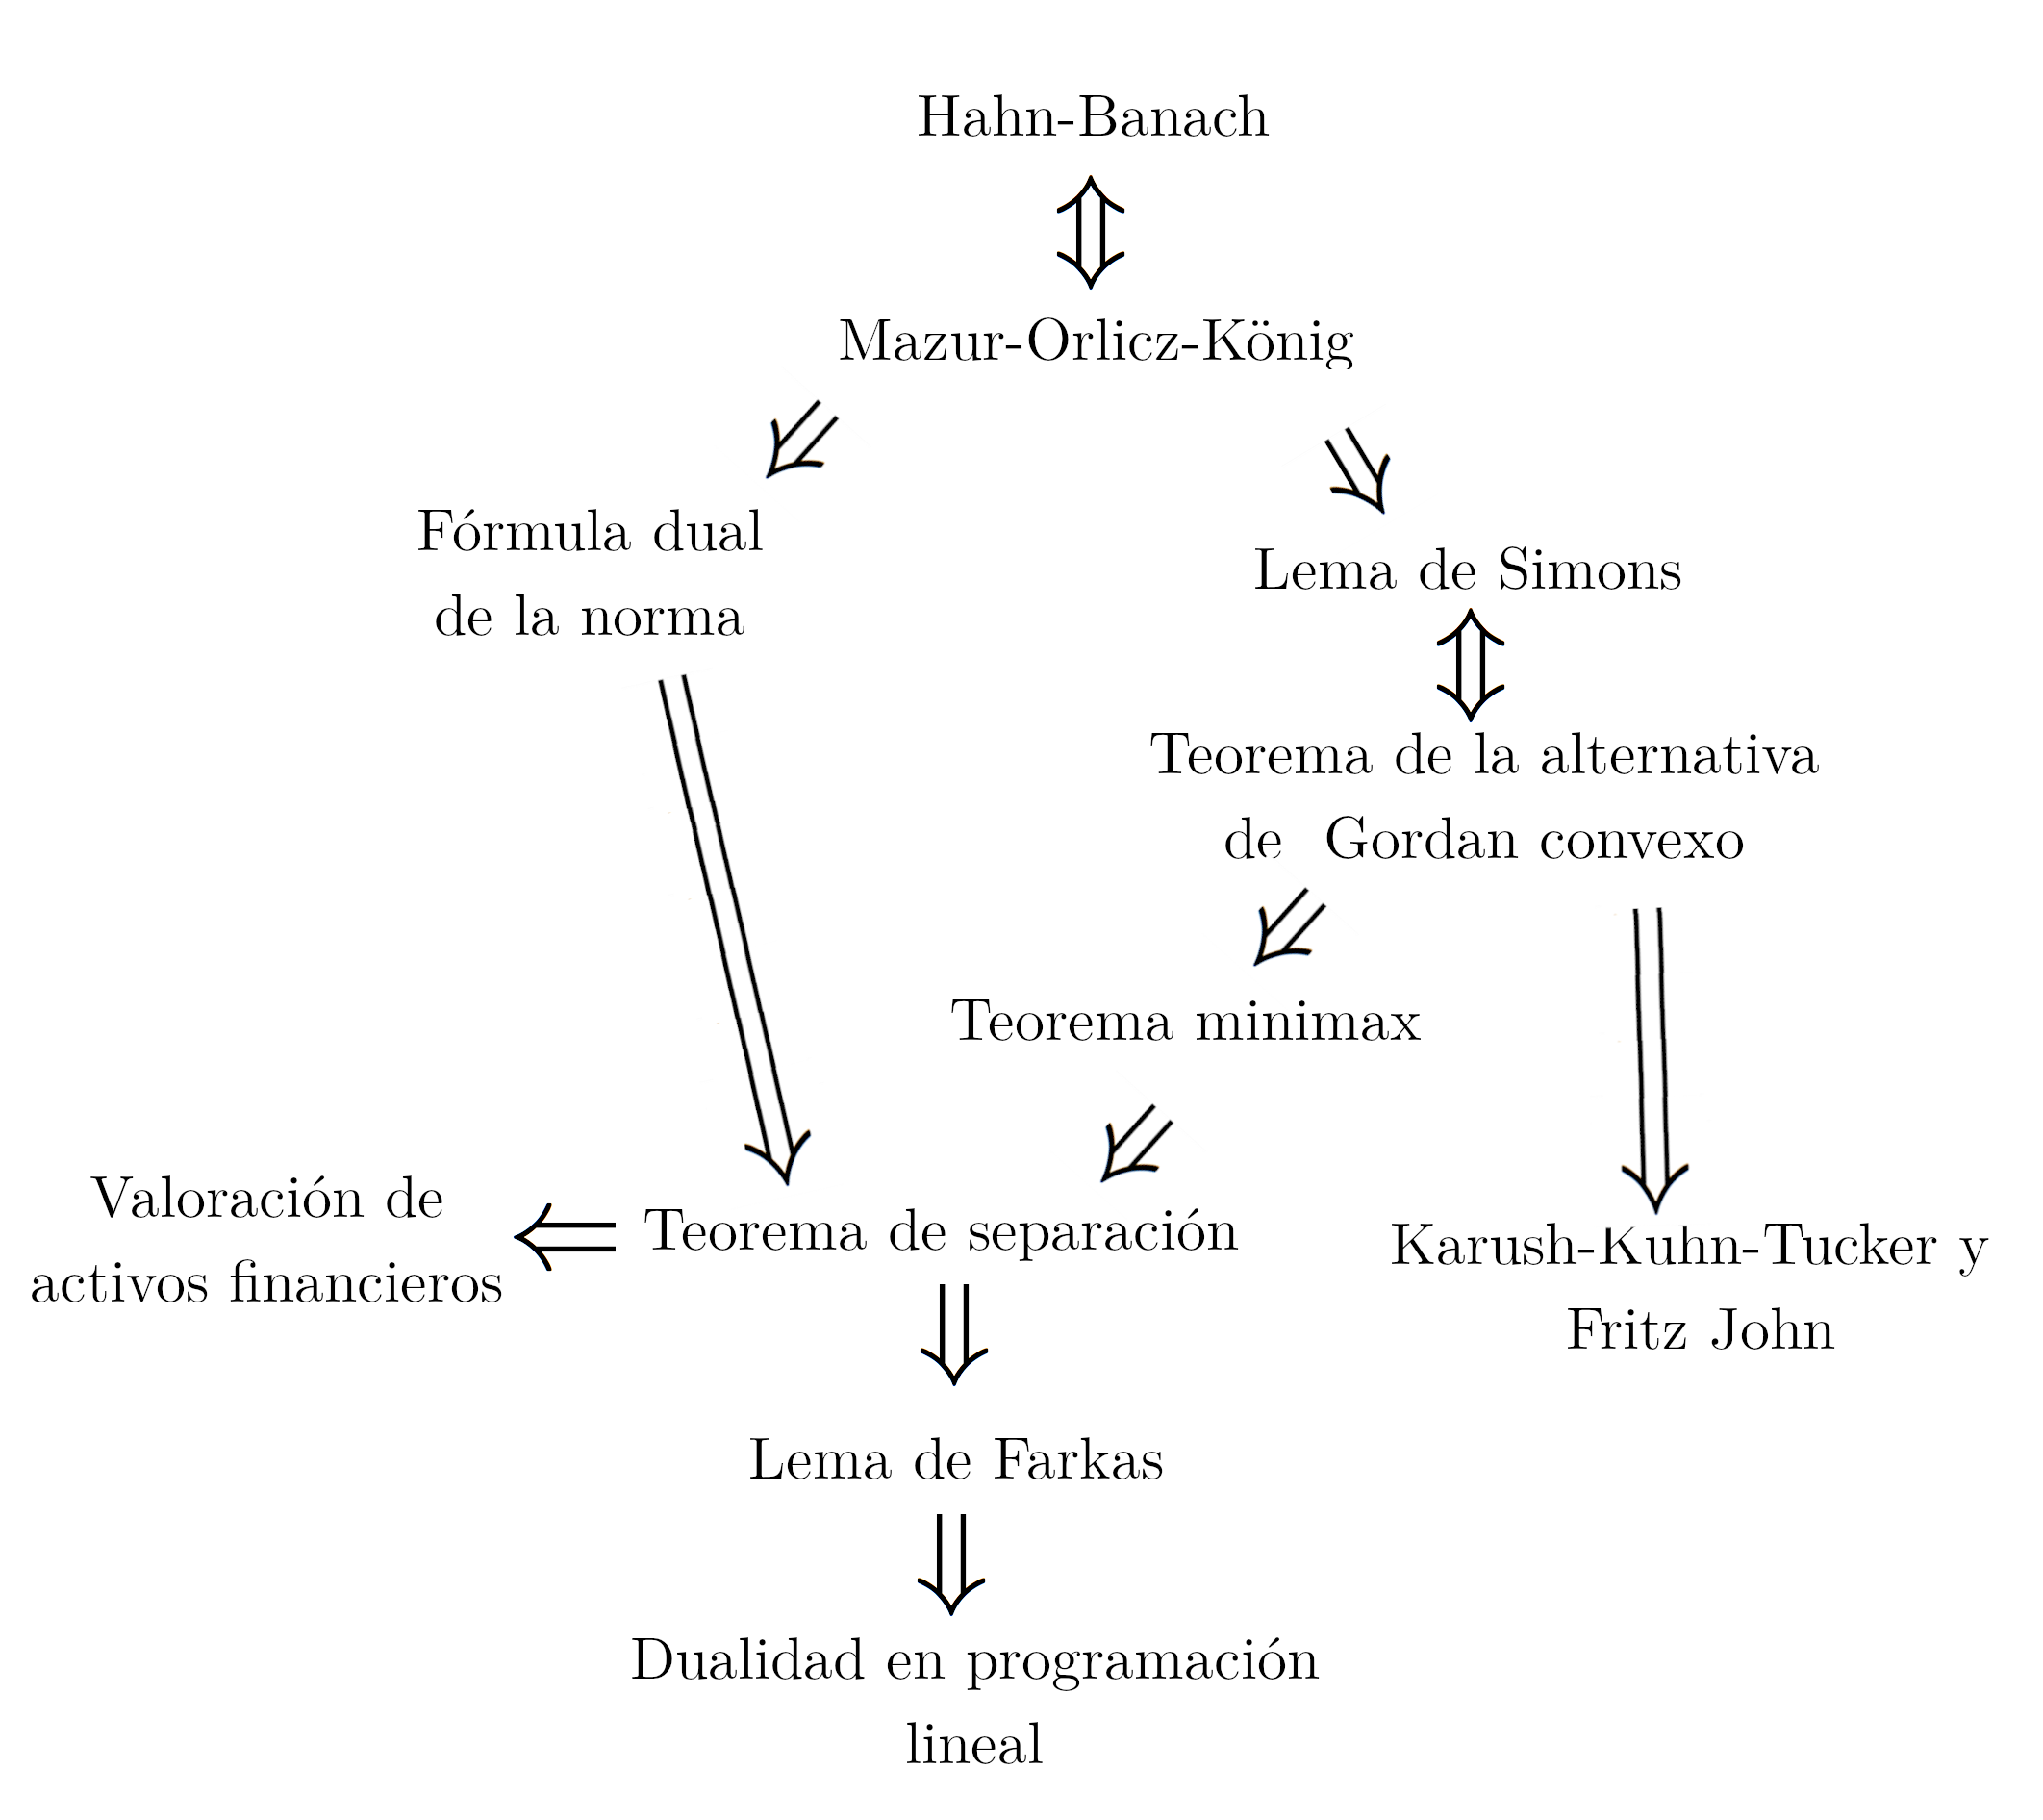
\includegraphics[width=0.9\linewidth]{imagenes/esquema.png}
	\label{fig:aux2}
\end{figure}

Como puede observarse, las técnicas son de carácter convexo y analítico funcional. En este sentido, han sido de gran utilidad el material de los textos \cite{Simons2008} y \cite{borwein}.
